\chapter{Estado del arte}
\label{cap:estadoDelArte}

% Corregido 01/01/2024
% Revisado 14/01/2024

Antes de entrar en el desarrollo del proyecto que en esta memoria se detalla me
gustaría introducir formalmente el concepto de ''ingeniería inversa'' o conocida
en el mundo de la informática como \textit{reverse engineering}. La ingeniería
inversa es el proceso de extraer conocimiento o el diseño de cualquier cosa que
el humano haya hecho. Por lo tanto, no es un concepto que solo acotemos dentro de
la ingeniería informática, sino que se puede aplicar a cualquier proceso ingenieril.
De hecho, este proceso es bastante similar al método científico, con la única diferencia
que la ingeniería inversa solo se aplica sobre cosas que ha hecho un humano y en el
método científico lo aplicamos en fenómenos naturales.

La ingeniería inversa es usada normalmente para obtener conocimiento desconocido o la
filosofía del diseño cuando esta información no está disponible, ya sea porque su
propietario ha decidido no compartirla o porque esta información está perdida o
destruida. \cite{alma991003132729706711}

La ingeniería inversa aplicada al \textit{software} es el mismo concepto, pero aplicada
a programa en su formato binario, con el objetivo de obtener el código fuente en un
lenguaje de programación concreto y así poder obtener información como el diseño del
programa. De hecho, la ingeniería inversa aplicada al \textit{software} requiere
diferentes artes: descifrado de códigos, resolución de puzzles, programación y análisis
lógico.

Las aplicaciones de la ingeniería inversa son muy variadas, pero podemos destacar dos
categorías: seguridad y desarrollo de \textit{software}.

Sus aplicaciones en seguridad son muy dispares, pero normalmente se le relaciona con
\textit{malware}, algoritmos criptográficos y auditorias sobre binarios.

Dentro del mundo del \textit{software} malicioso vemos que la ingeniería inversa se
utiliza en dos aspectos diferentes. Desde el punto de perspectiva de los que desarrollan
\textit{software} malicioso utilizan la ingeniería inversa para poder encontrar
vulnerabilidades en los programas que quieren infectar. En cambio, desde el punto de vista
de los desarrolladores de antivirus, utilizan la ingeniería inversa para poder diseccionar
y analizar cada programa malicioso.

También se puede aplicar ingeniería inversa sobre algoritmos criptográficos, de tal manera
que podamos averiguar que tan seguro es ese mensaje encriptado, o incluso en caso de utilizar
algoritmos basados en llaves, en los cuales la especificación del algoritmo de encriptación
es conocido, pero que cada implementación específica puede variar, encontrar vulnerabilidades
en estos algoritmos o el valor de las llaves.

Y por último, también la ingeniería inversa se aplica para realizar auditorias sobre binarios,
de tal manera que podamos detectar si un programa es seguro o no, encontrar sus vulnerabilidades
para poder corregirlas. Por lo tanto, cuanto mejores sean las herramientas de ingeniería inversa
que se apliquen, podremos encontrar con mucha más eficacia problemas de seguridad o funcionales
en \textit{software} propietario.

Como he mencionado con anterioridad, la ingeniería inversa también se aplica dentro del desarrollo
de \textit{software}, estas aplicaciones las podemos encontrar en diferentes etapas, por ejemplo
cuando disponemos de un \textit{software} propietario y la documentación es escasa, el uso de
herramientas de ingeniería inversa nos podrían ayudar a conseguir más interoperabilidad con
el \textit{software} propietario.

En conclusión, la ingeniería inversa es un proceso complejo y que requiere de muchas habilidades
y que sus aplicaciones son muy variadas, desde auditorias sobre binarios hasta mejorar
la interoperabilidad de dos programas. Pero en lo que inferimos claramente es que la
ingeniería inversa es necesaria para poder seguir mejorando la calidad del \textit{software}
que actualmente y en el futuro produciremos.

\section{Barreras de la ingeniería inversa}
\label{sec:barreras}

% Corregido 02/01/2024
% Revisado 14/01/2024

Como he mencionado, la ingeniería inversa no es un proceso sencillo y requiere de muchas
habilidades y conocimientos para poder aplicarla. En este apartado, me gustaría introducir
las diferentes barreras a nivel técnico que nos podemos encontrar a la hora de aplicar
ingeniería inversa sobre un programa informático. \cite{alma991004951313206711}

\begin{enumerate}
    \item \textbf{Diferencia entre Dominio de la Aplicación y Lenguajes de Programación}
        
        Traducir de conceptos de dominio (que es lo que quiero que haga mi aplicación) a
        un lenguaje de programación concreto y viceversa es un reto complejo, es decir, mapear
        conceptos del comportamiento del código a conceptos de dominio.

    \item \textbf{Concreción y abstracción}
        
        Cuando nos enseñan a programar, nos enseñan a abstraernos de los detalles de implementación
        y a pensar en términos de conceptos abstractos. Por lo tanto, cuando aplicamos ingeniería
        inversa, tenemos que hacer el proceso inverso, es decir, concretar los conceptos abstractos
        a partir de detalles de implementación.

    \item \textbf{Decadencia de la Estructura del Sistema}
        
        Muchos sistemas informáticos, a lo largo del tiempo y con el mantenimiento, han ido perdiendo
        su estructura original, por lo tanto, a la hora de aplicar ingeniería inversa, nos podemos
        encontrar con que el sistema no tiene una estructura clara, lo cual implica una dificultat añadida.

    \item \textbf{Disonancia Cognitiva}
        
        Los humanos pensamos en términos asociativos, mientras que los programas informáticos son expresiones
        jerárquicas formales. En consecuencia, supone un desafío a la hora de aplicar ingeniería inversa.

\end{enumerate}

\section{Fases de la ingeniería inversa}
\label{sec:fases}

% Corregido 02/01/2024
% Revisado 14/01/2024

Normalmente, la ingeniería inversa, cuando la queremos aplicar sobre programas informáticos, se divide en
cinco fases \cite{FasesIngineriaInversa}:

\begin{enumerate}
    \item \textbf{Recopilación de información}: esta fase consiste en recopilar toda la información posible
        sobre el programa que queremos analizar. Esta información puede ser desde el código fuente, la
        documentación, el manual de usuario, los binarios, etc.
    \item \textbf{Análisis estático}: una vez recopilada la información es hora de analizarla. En esta fase
        se analiza el código fuente, los binarios, la documentación, etc. El objetivo de esta fase es
        entender la estructura, el funcionamiento, la lógica y la organización interna del programa. Esta fase
        se caracteriza por no ejecutar el programa.
    \item \textbf{Análisis dinámico}: una vez hecho el análisis estático, es hora de ejecutar el programa
        y analizar su comportamiento. En esta fase se analiza el comportamiento del programa, como se comunica
        con el sistema operativo, como se comunica con otros programas, etc.
    \item \textbf{Desmontaje y decompilación}: para tener un análisis exhaustivo del programa, es necesario
        desmontar y descompilar el programa. El desmontaje consiste en obtener el código ensamblador del programa
        y la decompilación consiste en obtener el código fuente del programa.
    \item \textbf{Reconstrucción}: Esta etapa se hará en el caso de que sea necesario modificar el programa o
        mejorar la aplicación. Por ejemplo, en caso de detectar algún error durante las etapas anteriores, se
        puede modificar el programa para corregirlo.
\end{enumerate}

Cabe destacar, que en el contexto de este proyecto, el objetivo es poder automatizar o mejorar los resultados
de la fase de desmontaje y decompilación. Las otras fases son fases muy complejas y manuales que requieren
de una persona dedicada a ello.

\section{Historia de los Large Language Models}
\label{sec:historia}

% Corregido 14/01/2024
% Revisado 14/01/2024

El lenguaje es una de las habilidades más importantes que tenemos los seres humanos, y es
que gracias a esta habilidad podemos comunicarnos entre nosotros. Las máquinas no
tienen esta habilidad, a menos que las equipemos en algoritmos poderosos de inteligencia
artificial. Pero aun así, siempre ha sido un reto conseguir que las máquinas puedan leer,
escribir y comunicarse como los humanos.

\begin{figure}[H]
    \begin{center}
      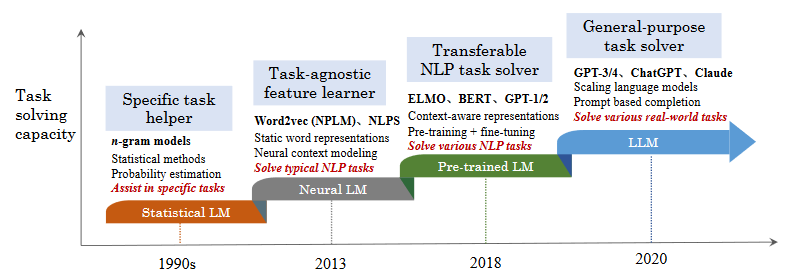
\includegraphics[width=15cm]{figuras/Capitulo_03/EvolutionLM.png}
    \end{center}
    \caption[Proceso de evolución de las cuatro generaciones de modelos lingüísticos (LM) desde la perspectiva de la capacidad de resolución de tareas.]{Proceso de evolución de las cuatro generaciones de modelos lingüísticos (LM) desde la perspectiva de la capacidad de resolución de tareas.(\cite{ZhaoWayneXin2023ASoL})}
    \label{fig:evolutionLM}
\end{figure}\

\textit{Lenguage modeling} (LM) es, a día de hoy, una de las mejores aproximaciones para conseguir
que las máquinas puedan entender el lenguaje humano. La investigación en las LM's se puede dividir
en cuatro tipos \cite{ZhaoWayneXin2023ASoL}:

\begin{enumerate}
    \item \textit{\textbf{Statistical language models (SLM)}}: Estos modelos están desarrollados basados en aprendizaje
        estadístico, y se basan en la probabilidad de que una secuencia de palabras aparezca en un texto. Los
        SLM se ha aplicado ampliamente para mejorar el rendimiento de las tareas de recuperación de información
        y el procesamiento del lenguaje natural. Sin embargo, los SLM tienen una gran limitación, es difícil
        estimar con precisión modelos lingüísticos de alto orden exponencial de probabilidades de transición.
    \item \textit{\textbf{Neural language models (NLM)}}: Los NLM se basan en redes neuronales para estimar la probabilidad
        de una secuencia de palabras. Los NLM han demostrado ser más efectivos que los SLM, pero tienen una gran
        limitación, y es que se necesitan grandes cantidades de datos de entrenamiento para poder obtener buenos
        resultados.
    \item \textit{\textbf{Pre-trained language models (PLM)}}: Los PLM son modelos lingüísticos preentrenados que se pueden
        utilizar para resolver tareas de procesamiento de lenguaje natural. Los PLM se entrenan en grandes conjuntos
        de datos de texto sin etiquetar, y se pueden utilizar para resolver tareas de procesamiento de lenguaje
        natural (NLP) específicas con un ajuste fino. Los PLM han demostrado ser muy efectivos en una amplia gama
        de tareas de NLP, pero tienen una gran limitación, y es que se necesitan grandes cantidades de datos de
        entrenamiento para poder obtener buenos resultados.
    \item \textit{\textbf{Large language models (LLM)}}: Los LLM son modelos lingüísticos que se entrenan en grandes conjuntos
        de datos de texto sin etiquetar y se pueden utilizar para resolver tareas de NLP específicas con un ajuste
        fino. Los LLM han demostrado ser muy efectivos en una amplia gama de tareas de NLP, y se pueden entrenar
        con conjuntos de datos de entrenamiento más pequeños que los PLM.
\end{enumerate}

En el caso de este proyecto, haremos hincapié en los LLM, ya que son los modelos que
se han utilizado para la realización de este proyecto. Típicamente, los \textit{Large
Language Models} se refiere a modelos de lenguajes que tienen cientos de billones de
parámetros, y que son entrenados con datos masivos de texto. Algunos de estos modelos
son GPT-3, PaLM, Galactica o LLaMA. Estos modelos han demostrado altas capacidades para
entender el lenguaje natural y resolver tareas complejas a través del lenguaje o texto.

Así mismo, dentro de los LLM estos han ido creciendo en tamaño y en cantidad de parámetros.
Para ilustrarlo, en la figura \ref{fig:evolutionLLM} podemos ver la evolución de los LLM a lo largo
del tiempo respecto a su tamaño y cantidad de parámetros.

\begin{figure}[H]
    \begin{center}
      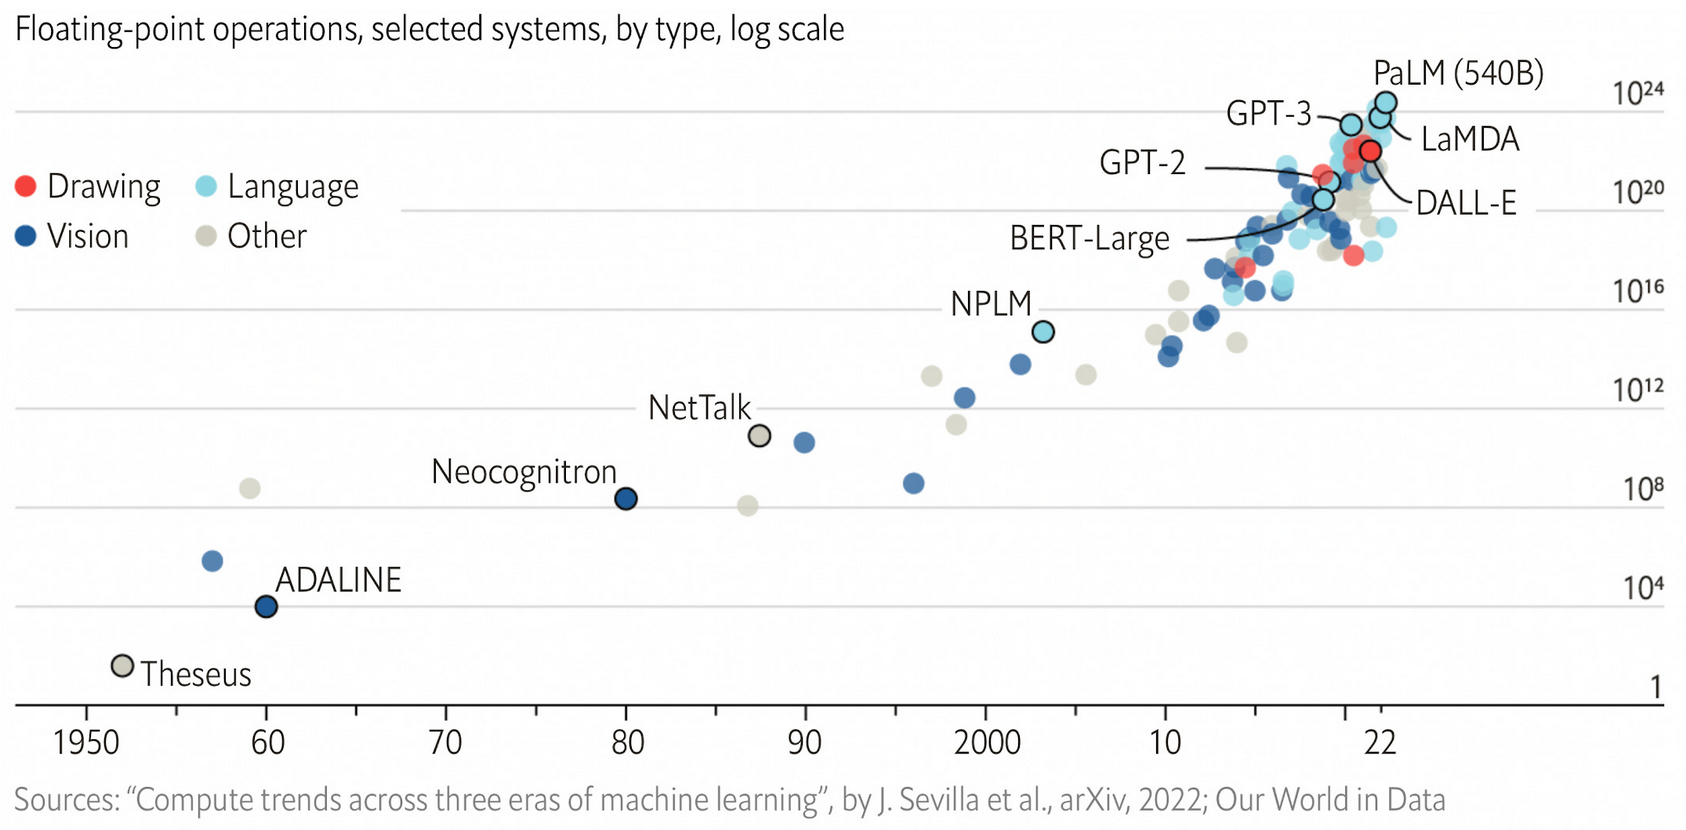
\includegraphics[width=15cm]{figuras/Capitulo_03/EvolutionLLM.png}
    \end{center}
    \caption[Operaciones de coma flotante por tipo en escala logarítmica]{Operaciones de coma flotante por tipo en escala logarítmica (\cite{EvolutionLLM})}
    \label{fig:evolutionLLM}
\end{figure}\

Pero lo que hace realmente interesante estos tipos de modelos es el concepto de
\textit{emergent abilities}, que nos viene a decir que hay habilidades que en
modelos pequeños no se observan, pero que en modelos grandes aparecen, es decir,
al haber augmentado el tamaño de los modelos a provocado que aprendan a hacer tareas
que los modelos más pequeños no han adquirido. Tres habilidades emergentes que se
han observado en los modelos grandes son:

\begin{itemize}
    \item \textbf{\textit{In-context learning}:} esta habilidad es la capacidad
        de generar el texto correcto a partir de una o más instrucciones en texto
        natural, más un conjunto de demostraciones de como se debe realizar la tarea.
        El modelo es capaz de realizar la tarea sin necesidad de entrenamiento previo.
        Esta habilidad fue introducida formalmente por GPT-3.
    \item \textbf{\textit{Instruction following}:} esta es la habilidad de seguir
        instrucciones por las cuales no se ha entrenado, es decir, si hacemos un
        \textit{fine-tuning} de un modelo con un conjunto de multitareas formateadas en
        lenguaje natural, el modelo es capaz de realizar las tareas sin necesidad de
        entrenamiento previo.
    \item \textbf{\textit{Step-by-Step reasoning}:} esta es la habilidad de resolver
        problemas de razonamiento complejos, concretamente en resolver tareas que
        requieren de múltiples pasos de razonamiento.
\end{itemize}

\subsection{Fine-tuning}
\label{subsec:fine_tuning}

% Corregido 02/01/2024
% Revisado 14/01/2024

\begin{wrapfigure}{r}{0.3\textwidth}
    \centering
    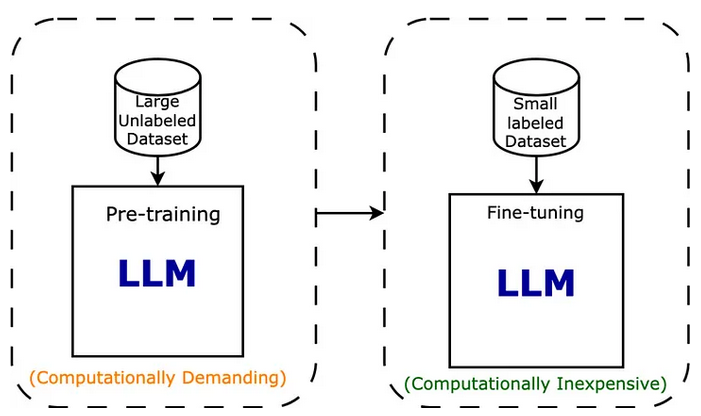
\includegraphics[width=0.3\textwidth]{figuras/Capitulo_03/TrainVSFinetuning.png}
    \caption[Entrenamiento versus \textit{fine-tuning}]{Entrenamiento versus \textit{fine-tuning} (\cite{SupervisedFineTuning})}
    \label{fig:finetuningVStraining}
\end{wrapfigure}

El \textit{fine-tuning} o en castellano ''ajuste fino'' es una técnica en la cual podemos ajustar
ciertos pesos en las capas de nuestra red neuronal, de tal manera que podamos afinar los
resultados de nuestro modelo para una tarea en específico. Esta técnica se parte de un
modelo preentrenado y se van ajustando las diferentes capas, en su totalidad o parcialmente,
con un conjunto de datos etiquetados. En esta técnica nos permite poder entrenar o ajustar los
modelos de manera eficiente y reduciendo los recursos computacionales y de memoria, pudiendo
incluso entrenar estos modelos en hardware de bajo coste o dispositivos comerciales para
uso doméstico.

Como he mencionado en la sección \ref{sec:historia}, los LLM tiene habilidades emergentes
que permiten que estos modelos puedan realizar tareas sin necesidad de entrenamiento previo.
Por lo tanto, en el \textit{fine-tuning} no buscamos enseñar al modelo como realizar una tarea sino
mejorar la capacidad de realizar dicha tarea. \cite{Finetuning}

\begin{figure}[H]
    \begin{center}
      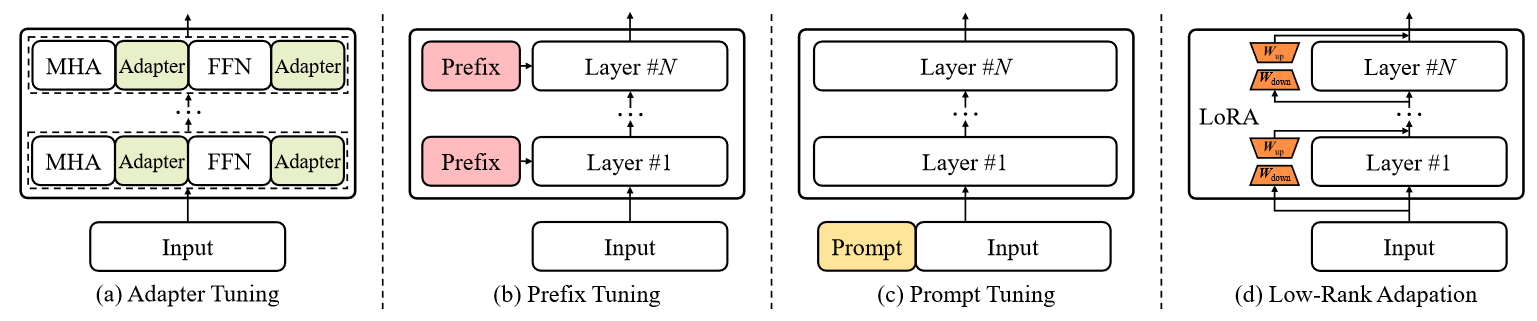
\includegraphics[width=15cm]{figuras/Capitulo_03/Finetuning.png}
    \end{center}
    \caption[Diagrama ilustrativo de los diferentes métodos de \textit{fine-tuning}]{Diagrama ilustrativo de los diferentes métodos de \textit{fine-tuning} (\cite{Finetuning})}
    \label{fig:finetuning}
\end{figure}

Dentro de las técnicas de \textit{fine-tuning} cabe destacar cinco métodos diferentes, aunque en
nuestro proyecto utilizaremos tan solo dos de ellos:

\begin{enumerate}
    \item \textit{\textbf{Prompt Tuning}}: El \textit{prompt tuning} es una técnica que consiste en
        añadir una pequeña cadena de texto al principio de la entrada, de tal manera que
        con esta cadena ajustamos y ordenamos las instrucciones para nuestra tarea en
        específico. Esta aproximación es la más sencilla y rápida y que normalmente aplicamos
        cuando por ejemplo interactuamos con ChatGPT.
    \item \textit{\textbf{Prefix-tuning}}: El \textit{prefix-tuning} es una técnica que consiste en
        añadir una pequeña cadena de texto al principio de cada capa del modelo neuronal.
        Con esta capa lo que intentamos es ajustar y ordenar las instrucciones para nuestra
        tarea en específico.
    \item \textit{\textbf{Adapter}}: este método incorpora módulos pequeños de redes neuronales,
        llamados adaptadores, que se conectan a las capas de salida de los modelos
        preentrenados. De tal manera que el proceso de \textit{fine-tuning} se optimizan los
        adaptadores para la tarea en específico mientras los del modelo original
        quedan congelados. De esta manera se consigue reducir de manera considerable
        el número de parámetros entrenables durante el \textit{fine-tuning}.
    \item \textit{\textbf{Low rank adaptation (Lora)}}: este método lo que hace es 
        reducir el número de parámetros haciendo que la matriz de actualización sea de rango bajo.
        Consideremos una matriz de actualización $W$ y el proceso de \textit{fine-tuning}
        $W\leftarrow W + \bigtriangleup W$. LoRa propone congelar la matriz original
        $W\in \mathbb{R}^{m\times n}$ y convertir el proceso de actualización ($\bigtriangleup W$)
        bajando el rango de la matriz y descomponiéndola, de tal manera que nos queda
        $\bigtriangleup W = A\cdot B^T$ donde $A\in \mathbb{R}^{m\times k}$ y $B\in \mathbb{R}^{n\times k}$.
        \cite{ZhaoWayneXin2023ASoL}
    \item \textit{\textbf{QLoRa}}: este método reduce notablemente la cantidad de memoria
        que se necesita para poder hacer el \textit{fine-tuning} de los modelos. Este método
        utiliza la técnica de \textit{LoRa} pero con una matriz de actualización cuantizada. De tal
        manera que la matriz de actualización se puede representar con un número de bits
        mucho menor.\cite{DettmersTim2023QEFo}
\end{enumerate}

\begin{figure}[H]
    \begin{center}
      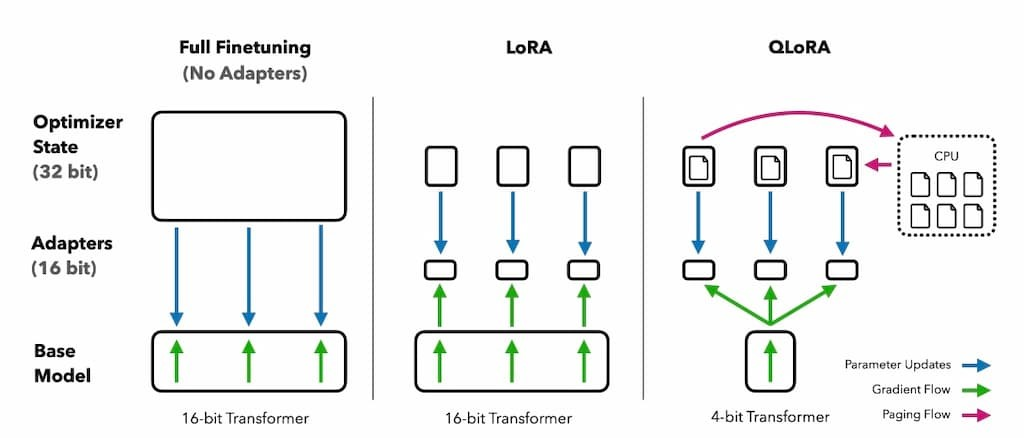
\includegraphics[width=12cm]{figuras/Capitulo_03/QLoRa.jpg}
    \end{center}
    \caption[Diagram ilustrativo de como funciona \textit{LoRa} y \textit{QLoRa}]{Diagram ilustrativo de como funciona \textit{LoRa} y \textit{QLoRa} (\cite{DettmersTim2023QEFo})}
    \label{fig:qlora}
\end{figure}

\subsection{Cuantización de modelos}
\label{subsec:cuantizacion}

% Corregido 14/01/2024
% Revisado 14/01/2024

La cuantización surge por la necesidad de poder ejecutar modelos de redes neuronales,
que cada vez son mucho más grandes y complejos, en dispositivos con recursos limitados.
La idea básica que hay detrás de la cuantización es la de comprimir, es decir, reducir
la precisión numérica de los parámetros del modelo para obtener representaciones más
compactas que requieren menos bits y, por lo tanto, menos memoria.

Un símil lo podríamos encontrar en la música, donde podemos encontrar diferentes formatos
con diferentes precisiones que permiten comprimir la música y reducir el tamaño del archivo.
Por ejemplo, el formato WAV tiene una precisión de 16 bits, mientras que el formato MP3
tiene una precisión de 8 bits.

Volviendo al mundo de las redes neuronales, la mayoría de redes neuronales utilizan números
de coma flotante de 32 bits para representar los parámetros del modelo. Pero la cuantización
puede reducir la precisión de los parámetros a 8 bits. Para lograrlo se mapean los grandes
rangos de valores de punto flotante a rangos más pequeños de valores enteros.

\begin{itemize}
    \item \textit{4-bit NormalFloat Quantization} \cite{DettmersTim2023QEFo}
    \item \textit{Double Quantization} \cite{DettmersTim2023QEFo}
    \item \textit{4-bit Floating Point} \cite{DettmersTim2023QEFo}
    \item \textit{El algoritmo GPTQ} \cite{DettmersTim20218OvB}
    \item \textit{8-bit optimizers via block-wise quantization} \cite{FrantarElias2022GAPQ}
\end{itemize}

En el contexto de este proyecto, nos centraremos en la cuantización \textit{4-bit
NormalFloat Quantization} que es la que se ha utilizado para poder cuantizar los
modelos de lenguaje que se han utilizado para la realización de este proyecto.

Cabe destacar que la cuantización de modelos conlleva una pérdida de precisión y, por
lo tanto, su uso puede provocar que para ciertas tareas el resultado no sea lo esperado.

\section{Soluciones y alternativas existentes}
\label{sec:alternativas}

% Corregido
% Revisado 14/01/2024

Actualmente, en el mercado podemos encontrar diferentes herramientas o programas llamados
decompiladores o reversores los cuales tienen la capacidad de convertir un ejecutable
en un código C aproximado llamado normalmente por estas herramienta como pseudocódigo.

Así mismo, la mayoría de estas herramientas están más orientadas a la generación de un
código ensamblador más ``amigable'' y que mayoritariamente siempre necesitara intervención
para que pueda ser más legible y así ayudar en procesos de depuración.

Algunas de estas herramientas son:

\begin{itemize}
    \item \bf IDA Pro \cite{IDAProWebSite}
    \item \bf Ghidra \cite{GhidraSite}
    \item \bf AllyDbg \cite{OllyDbgSite}
\end{itemize}

En la próxima sección detallaremos un poco más la herramienta IDA Pro en su vertiente
gratuita llamada IDA Free \cite{IDAFreeSite}, ya que esta es la más usada para aplicar
ingeniería inversa.

\subsection{IDA Pro}
\label{subsec:IDA_pro}

% Corregido 14/01/2024
% Revisado 14/01/2024

IDA o \textit{Interactive Disassembler} es un desensamblador que es utilizado para
ingeniería inversa. IDA soporta una variedad de formato de ejecutables para diferentes
procesadores y sistemas operativos. También es usado como depurador para ejecutables
del tipo Windows PE, Mac OS X, Mach-O y Linux ELF\cite{IDAPro_Wikipedia}. Aunque
nativamente IDA no tiene decompilador, en sus últimas versiones dispones de un \textit{plug-in}
que nos brinda esta funcionalidad. Cabe destacar que este plug-in es un decompilador
basado en \textit{cloud}, es decir, requiere de conexión a internet para poder generar
un pseudocódigo a partir de un ejecutable.

Para poder analizar en más profundidad esta herramienta he hecho diferentes pruebas
con códigos muy sencillas para poder comprobar que tipo de solución nos da esta
herramienta. Para ello he utilizado el código \ref{cod:binarySearch}, donde se observa
la implementación del algoritmo de búsqueda binaria en código C.

\begin{mycode}
    \begin{minted}[fontsize=\scriptsize]{c}
/** Recursive implementation
* \param[in] arr array to search
* \param l left index of search range
* \param r right index of search range
* \param x target value to search for
* \returns location of x assuming array arr[l..r] is present
* \returns -1 otherwise
*/
int binarysearch1(const int *arr, int l, int r, int x)
{
    if (r >= l)
    {
        int mid = l + (r - l) / 2;

        // If element is present at middle
        if (arr[mid] == x)
            return mid;

        // If element is smaller than middle
        if (arr[mid] > x)
            return binarysearch1(arr, l, mid - 1, x);

        // Else element is in right subarray
        return binarysearch1(arr, mid + 1, r, x);
    }

    // When element is not present in array
    return -1;
}

/** Iterative implementation
* \param[in] arr array to search
* \param l left index of search range
* \param r right index of search range
* \param x target value to search for
* \returns location of x assuming array arr[l..r] is present
* \returns -1 otherwise
*/
int binarysearch2(const int *arr, int l, int r, int x)
{
    int mid = l + (r - l) / 2;

    while (arr[mid] != x)
    {
        if (r <= l || r < 0)
            return -1;

        if (arr[mid] > x)
            // If element is smaller than middle
            r = mid - 1;
        else
            // Else element is in right subarray
            l = mid + 1;

        mid = l + (r - l) / 2;
    }

    // When element is not present in array
    return mid;
}
    \end{minted}
    \caption[Búsqueda binaria en su forma iterativa y recursiva]{Búsqueda binaria en su forma iterativa y recursiva (\cite{BinarySearchGitHub})}
    \label{cod:binarySearch}
\end{mycode}

Compilamos el código y con el ejecutable que nos genera se lo damos a IDA Free y
utilizando el plug-in de decompilador basado en \textit{cloud} generamos un
pseudocódigo de los métodos que encontramos en el código \ref{cod:binarySearch}.
En la figura \ref{fig:IDAPro_binaryseacrh1} podemos observar la función \textit{binarysearch1()}
y en la figura \ref{fig:IDAPro_binaryseacrh2} podemos observar la función \textit{binarysearch2()}.

\begin{figure}[H]
    \begin{center}
      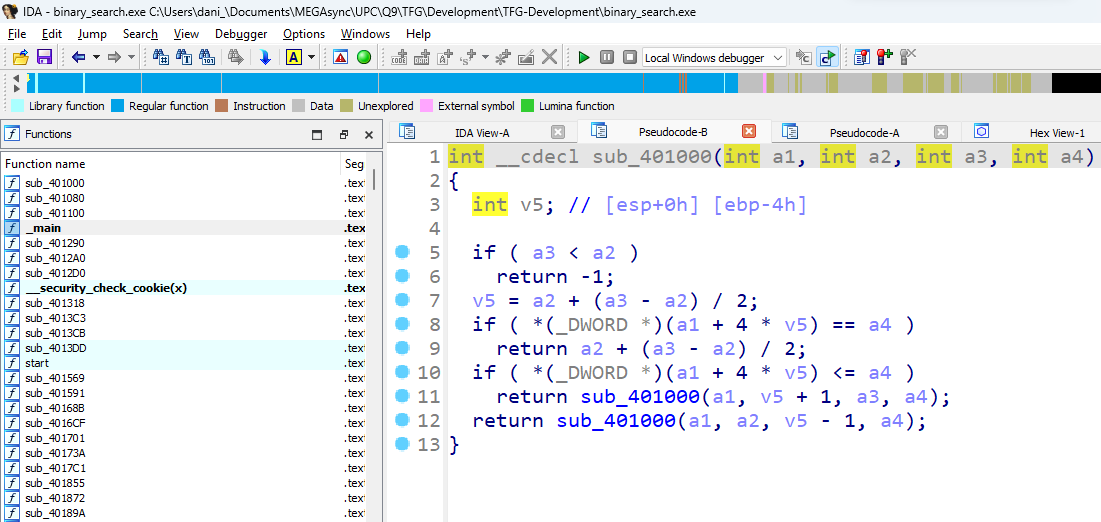
\includegraphics[width=15cm]{figuras/Capitulo_03/IDAPro_binaryseacrh1.png}
    \end{center}
    \caption[Captura de pantalla de IDA Free con el pseudocódigo generado para la funcion \textit{binaryseacrh1}]{Captura de pantalla de IDA Free con el pseudocódigo generado para la funcion \textit{binaryseacrh1} (Elaboración propia)}
    \label{fig:IDAPro_binaryseacrh1}
\end{figure}\

\begin{figure}[H]
    \begin{center}
      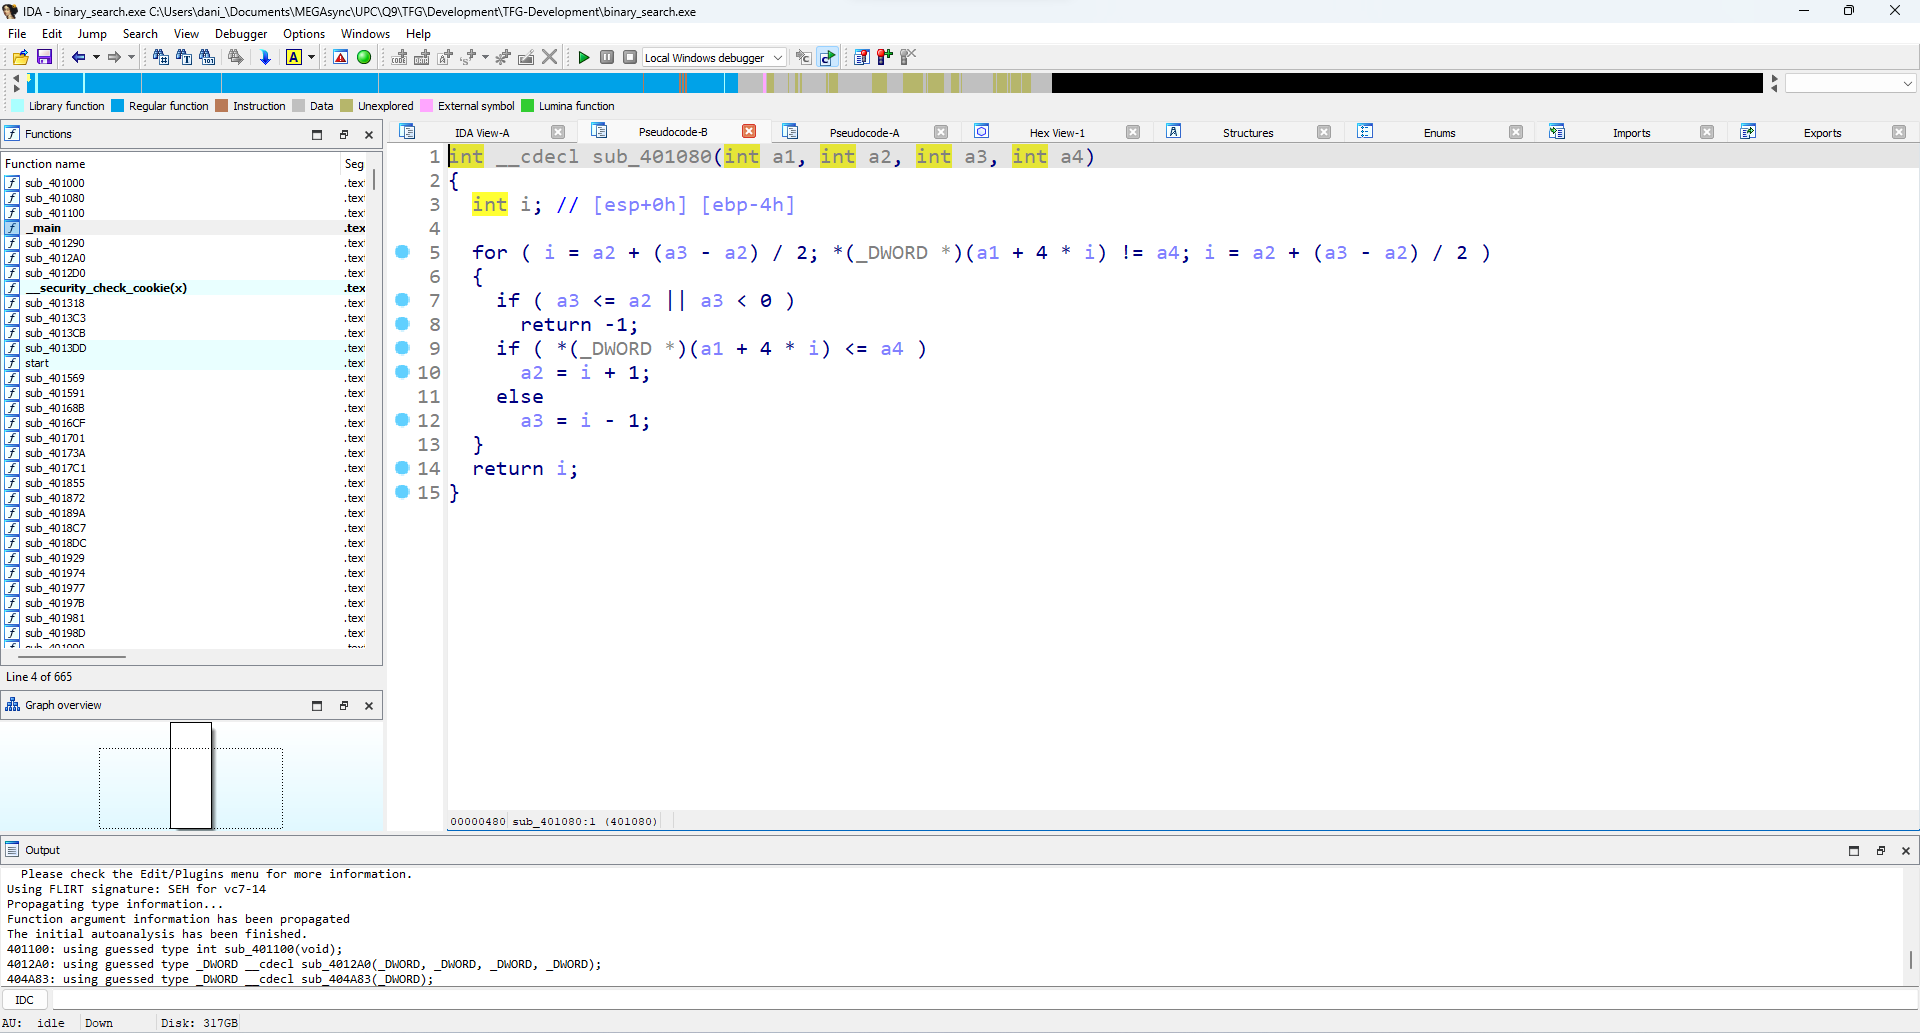
\includegraphics[width=15cm]{figuras/Capitulo_03/IDAPro_binaryseacrh2.png}
    \end{center}
    \caption[Captura de pantalla de IDA Free con el pseudocódigo generado para la funcion \textit{binaryseacrh2}]{Captura de pantalla de IDA Free con el pseudocódigo generado para la funcion \textit{binaryseacrh2} (Elaboración propia)}
    \label{fig:IDAPro_binaryseacrh2}
\end{figure}\

Como se puede observar, el pseudocódigo generado es bastante legible y se puede
entender el funcionamiento básico de los métodos. Pero también se puede observar
que el pseudocódigo generado no es capaz de dar nombre de funciones o de variables
que sean representativos. Así mismo, observamos que en algunas comprobaciones la
legibilidad del código es bastante pobre y dificulta en muchos casos el entendimiento
eficaz de la funcionalidad del código.

\section{Ética y legalidad}
\label{sec:etica_legalidad}

% Corregido 14/01/2024
% Revisado 14/01/2024

Cuando inicie este proyecto, una de las primeras peguntas que me hice fue: si conseguimos
generar código a partir de un ejecutable, ¿sería legal? ¿Sería ético? ¿Qué implicaciones
legales y éticas tendría?

Creo que es importante reflexionar e indagar más sobre este asunto, ya que, como estudiante
de ingeniería, uno ha de ser consciente de las repercusiones de los proyectos que desarrolla y
de las implicaciones que tiene en la sociedad. Así mismo, también es crucial saber que las
técnicas aplicadas en este proyecto son legales o no.

Para poder responder a estas preguntas, me gustaría empezar por la ética. Creo que muchos, cuando
lean esta memoria, se sentirán identificados cuando de pequeños cogíamos juguetes o aparatos electrónicos
para desmontarlos y poder ver como funcionaban. En aquel momento, desconocíamos que lo que estábamos
haciendo era aplicar ingeniería inversa, ¿pero quiere decir esto que lo que hacíamos era ilegal o inmoral?

El ser humano, por naturaleza, es curioso y siempre ha tenido la necesidad de entender como funcionan
las cosas, es algo innato y que nos ha ayudado a tener las tecnologías que hoy en día tenemos. Por lo tanto,
creo que lo importante es con qué finalidad se hace. Si lo hacemos con la finalidad de aprender y entender
como funcionan las cosas para poder crear nuevos productos o mejorar los existentes, creo que es algo
positivo y necesario.

Por dar un ejemplo ilustrativo, en los años 80's IBM dominaba el mercado de los ordenadores personales
con su IBM PC gracias a su BIOS\footnote{\textit{Basic Input Output System} es el primer programa que se
ejecuta cuando encendemos un ordenador. La función principal es iniciar y probar el \textit{hardware}
del sistema y cargar un gesto de arranque o un sistema operativo.}, en aquel momento IBM era la único empresa
que fue capaz de crear un programa que se encargara de gestionar el \textit{hardware} del ordenador y que
permitiera cargar un sistema operativo. Por lo tanto, IBM tenía el monopolio de los ordenadores personales
e IBM se encargaba de proteger su monopolio amenazando a cualquier otra empresa que intentara clonar su sistema.
Phoenix Technologies, decidió aplicar la técnica de la habitación limpia, la cual consistía en tener dos grupos
de ingenieros totalmente desvinculados, donde uno se encargaba de estudiar en profundidad la BIOS de IBM para
transmitírselo al segundo grupo, sin especificar detalles técnicos o de código y que, por lo tanto, pudieran
crear un sistema que se comportara de igual manera programada desde cero.

En este caso, gracias a un sistema basado en la ingeniería inversa, se pudo crear un sistema que se comportaba
de la misma manera que el sistema de IBM, pero programado desde cero y, por lo tanto, acabar con el monopolio
de IBM, lo cual fue muy beneficioso para el mercado y para los consumidores. \cite{IngenieriaInversa}

Por lo que respecta a la legalidad de la ingeniería inversa, creo que es un tema más complejo y que depende
mucho de la legislación de cada país. En el caso de España, el Real Decreto Legislativo 1/1996, de 12 de abril,
por el que se aprueba el texto refundido de la Ley de Propiedad Intelectual, en su artículo 100, que establece
los límites de explotación de la obra, en su apartado 3:

\begin{quote}
\textit{''El usuario legítimo de la copia de un programa estará facultado para observar, estudiar o
verificar su funcionamiento, sin autorización previa del titular, con el fin de determinar las ideas
y principios implícitos en cualquier elemento del programa, siempre que lo haga durante cualquiera de
las operaciones de carga, visualización, ejecución, transmisión o almacenamiento del programa que tiene
derecho a hacer\cite{LeyPropiedadIntelectual}''}
\end{quote}

Como se puede observar, la ley contempla que nosotros como usuarios podamos analizar e indagar en el funcionamiento
de un programa informático que legítimamente hemos adquirido y dentro de los términos de uso, es decir, aplicar
ingeniería inversa.

A pesar de que hay muchos casos a contemplar que se van fuera del marco de este proyecto y de muchas más leyes
que entran en juego a la hora de aplicar ingeniería inversa, podemos concluir que mientras estos programas se hayan
adquirido legalmente, podremos aplicar ingeniería inversa sobre estos, siempre y cuando la finalidad no sea copiar,
sino entender el funcionamiento de un producto adquirido.
